\section{Performance evaluation}
\label{sec:performance}
As part of the midterm milestone meeting the baseline performance of the processor was re-evaluated. After that the size of the cache was increased and the cache mapping mechanism was improved to give it the ability to cache the full 4MB of the main memory. This section discusses the results of these experiments.

\subsection{Baseline}
\Cref{tab:baselinebench,tab:baselineperformance} show a comparison of reported performance versus measured performance. All the benchmarks were run on the FPGA to obtain the measured benchmark scores of \cref{tab:baselinebench}. The opcodes benchmark was simulated using Questasim. All the measured benchmarks are close to those reported in the project manual.
\begin{table}[H]
\centering
\begin{tabular}{lll}
\hline
Name       & Benchmark score (reported) & Benchmark score (measured) \\ \hline
opcodes    & verified                   & verified                   \\
cjpeg      & 29.740140                  & 29.316406                            \\
divide     & 264.820001                 & 274.860369                            \\
multiply   & 149.492876                 &   155.283095                          \\
pi         & 845.277552                 &   845.294532                          \\
fir        & 187.411039                 &  187.537571                           \\
rsa        & 563.89053                  &   577.504991                          \\
ssd        & 797.170350                 &  860.871400                           \\
ssearch    & 457.727967                 &  475.458147                           \\
susan      & 910.498879                 &  916.969617                           \\
bench\_all & 4323.096258                &  4323.096128                          \\ \hline
\end{tabular}
\caption{Comparison of benchmark scores reported by project manual and measured benchmark scores. All scores in million cycles.}
\label{tab:largecachebench}
\end{table}
For \cref{tab:baselineperformance} the steps from the project manual were followed to generate the specifications. For area 9 $A_{FIFO16/RAMB16}$ and 2022 $A_{SLICE}$ were found which resulted in an area of 514.5 $A_{CLB}$ when the weights of $A_{FIFO16/RAMB16} = A_{CLB}$ and $A_{SLICE} = A_{CLB}/4$ from the project manual were used. For frequency the minimum clock period was found to be \SI{23.686}{\nano\second} which resulted in \SI{42.219}{\mega\hertz} as the maximum frequency. Power was estimated for the pi benchmark with \SI{1}{\milli\second} simulation time which resulted in a total power estimate of \SI{0.698}{\watt}. A more detailed power analysis can be found in \cref{fig:baselinepower}. The power, area and frequency totals are all equal to those reported in the project manual. The more detailed power analysis in \cref{fig:baselinepower} is not exactly the same but very similar to the values found in the manual.
\begin{table}[H]
\centering
\begin{tabular}{lll}
\hline
Attribute       & Reported & Measured \\ \hline
Power    &  \SI{0.698}{\watt}        &   \SI{0.698}{\watt}                \\
Area     &       541.5 $A_{CLB}$            & 541.5 $A_{CLB}$             \\
Frequency    &   \SI{42.219}{\mega\hertz}           &  \SI{42.219}{\mega\hertz}                         \\\hline
\end{tabular}
\caption{Comparison of baseline specifications reported by project manual and measured specifications.}
\label{tab:baselineperformance}
\end{table}

\begin{figure}[H]
\centering
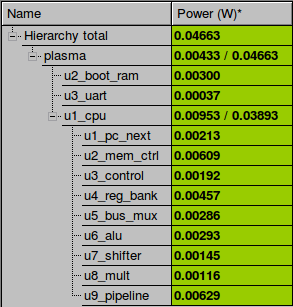
\includegraphics{../resource/baselinepower}
\caption{Detailed power analysis by hierarchy for baseline processor.}
\label{fig:baselinepower}
\end{figure}

\subsection{Larger cache}
\begin{table}[H]
\centering
\begin{tabular}{llll}
\hline
Name        & \SI{4}{\kilo\byte} & \SI{8}{\kilo\byte}& \SI{16}{\kilo\byte}\\ \hline
cjpeg       & 29.316406                 & 28.455434               &           \\
divide      & 274.860369                & 265.116735               &            \\
multiply    &   155.283095              & 150.094662               &            \\
pi          &   845.294532              &  844.614099              &            \\
fir         &  187.537571               &  186.518289               &            \\
rsa         &   577.504991              &  574.562761               &            \\
ssd         &  860.871400               & 833.108159                &            \\
ssearch     &  475.458147               &  448.907365               &            \\
susan       &  916.969617               & 914.132525                &            \\
bench\_all  &  4323.096128              & 4245.510029               &            \\ \hline
\end{tabular}
\caption{Comparison of benchmark scores reported by project manual and measured benchmark scores. All scores in million cycles.}
\label{tab:baselinebench}
\end{table}

\subsection{Improved cache mapping}